
%%%%%%%%%%%%%%%%%%%%%%%%%%%%%%%%%%%%%%%%%%%%%%%%%%%%%%%
%%              Supplementary Content                %%
%%%%%%%%%%%%%%%%%%%%%%%%%%%%%%%%%%%%%%%%%%%%%%%%%%%%%%%
%------------------------------------------------
\section{Supplementary content}
%------------------------------------------------
\subsection{Training challenges}
%------------------------------------------------
\begin{frame}[t]
    \frametitle{Training the model}
	%
	There are several challenges associated with hyperparameter optimization\\
	%
    \begin{columns}[t] % The "c" option specifies centered vertical alignment while the "t" option is used for top vertical alignment
		
        \begin{column}{.5\textwidth} % Left column and width
        \only<1->{
			\begin{itemize}
				\item The number of epochs can be tuned using \textit{early stopping}%
				\item This is a form of \textit{regularization} to reduce over-fitting%
			\end{itemize}
        }%
        \only<3->{
			~~~However,\\
			\uncover<4->{
				~~~1) Other hyperparameters to tune
				\begin{itemize}
					\item Dropout%
					\item Training batch size%
					\item Activation function(s)%
				\end{itemize}
			}%
            \uncover<5->{~~~2) Training can be \emphasis{expensive}}\\
            \uncover<6->{~~~3) Backpropagation is \emphasis{stochastic}}
        }%
    
        \end{column}
    
        \begin{column}{.5\textwidth} % Left column and width
    
            \vspace{-1.5em}
            \begin{figure}
                \centering
                \only<1>{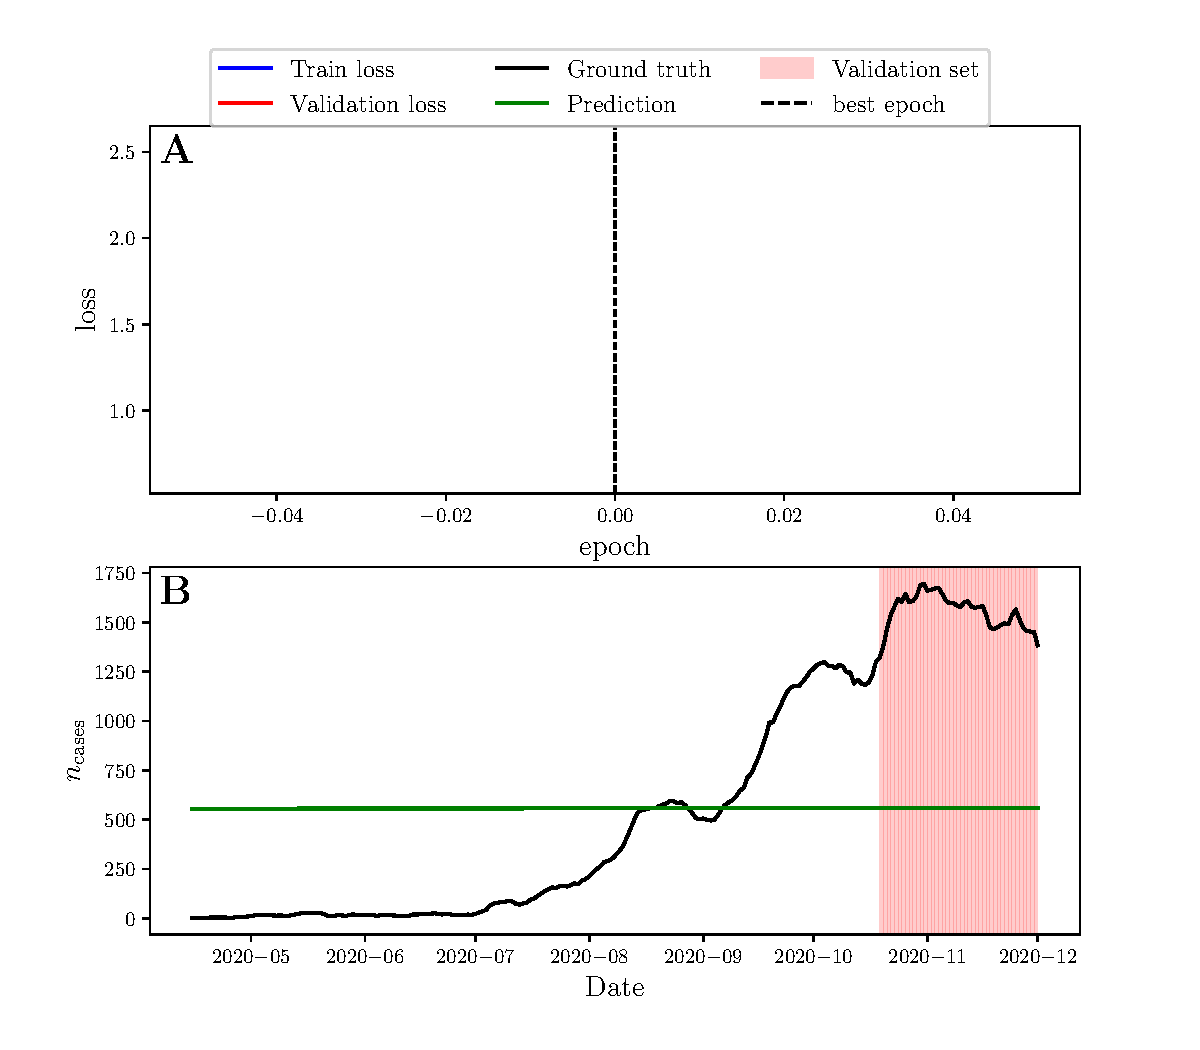
\includegraphics[width=0.9\textwidth]{training/epoch_0.pdf}}%
                \only<2>{
					\begin{animateinline}[autoplay,width=0.9\textwidth]{8}
						\ifshowanimations
							\multiframe{52}{i=0+5}{%
								\includegraphics{training/epoch_\i.pdf}
							}
						\else
							\multiframe{1}{i=262+0}{%
								\includegraphics{training/epoch_\i.pdf}
							}
						\fi
					\end{animateinline}%
                }%
                \only<3->{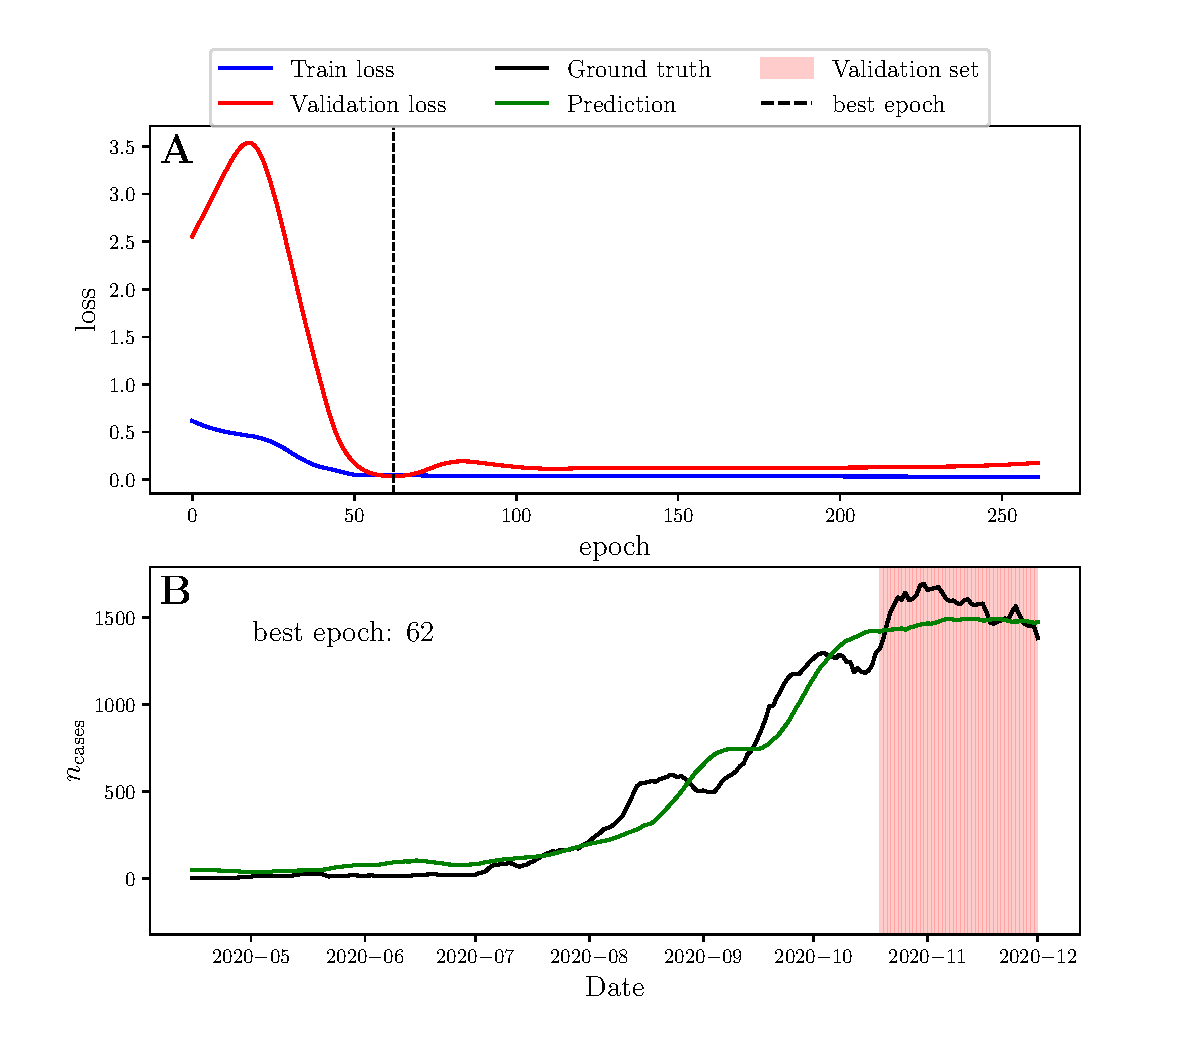
\includegraphics[width=0.9\textwidth]{training/final_model.pdf}}%
                \vspace{-0.75em}
                \caption{Effect of number of epochs on testing loss}
            \end{figure}%
        \end{column}
    \end{columns}
        
\end{frame}
%------------------------------------------------
\subsection{Hyperparameter tuning results}
%------------------------------------------------
\begin{frame}[t,noframenumbering]
	\frametitle{Hyperparameter tuning: other hyperparamters}
	\tikzstyle{background grid}=[draw, black!50,step=.5cm]
	%
	We can use StoMADS to solve such hyperparameter optimization problems \ifshowcitations\footpartcite{Khalil2021}\fi\\
	%
	\tikzstyle{background grid}=[draw, black!50,step=.5cm]
	\begin{tikzpicture}[remember picture, overlay] %show background grid, 
		% Put the graphic inside a node. This makes it easy to place the
		% graphic and to draw on top of it. 
		% The above right option is used to place the lower left corner
		% of the image at the (0,0) coordinate. 
		\node [inner sep=0pt,above right, opacity=1.0]  at (-0.01\textwidth,-0.7\textheight) (error) 
			{
				\only<1>{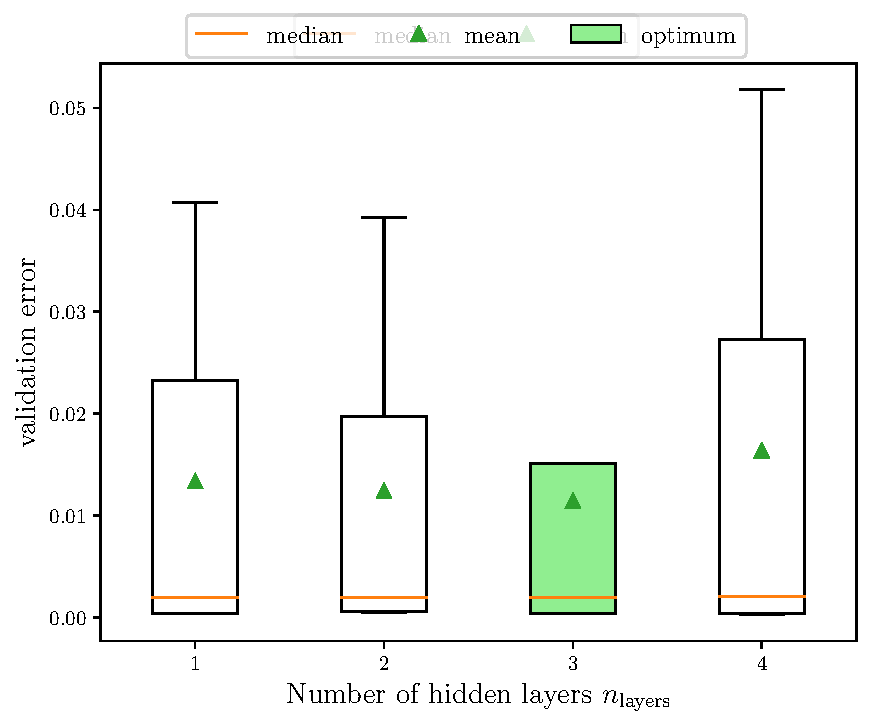
\includegraphics[width=0.5\textwidth]{box_plots/boxplot_n_layers_opt.pdf}}%
				\only<2>{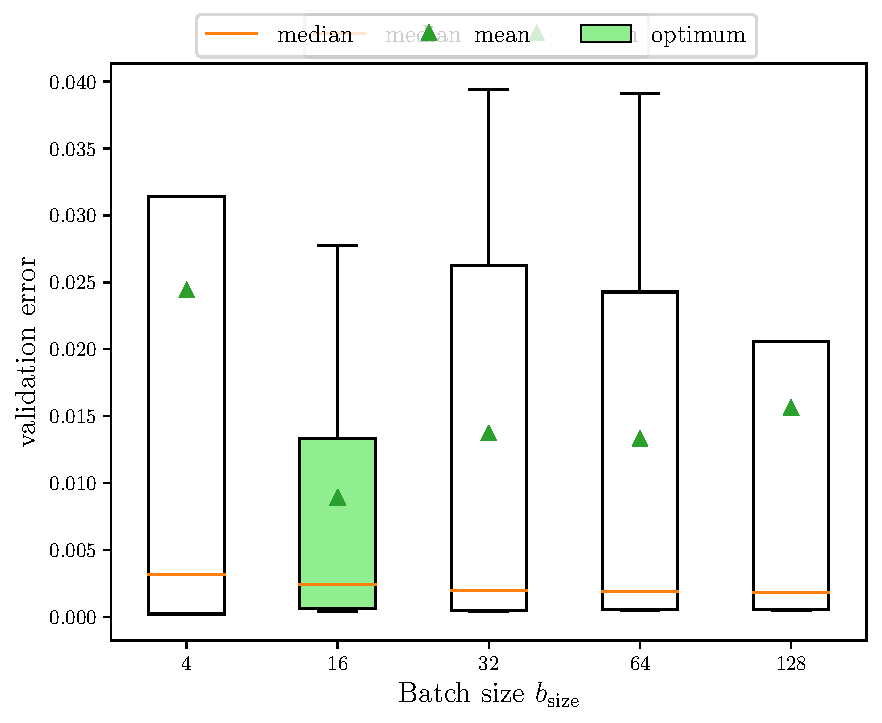
\includegraphics[width=0.5\textwidth]{box_plots/boxplot_batch_size_opt.pdf}}%
				\only<3>{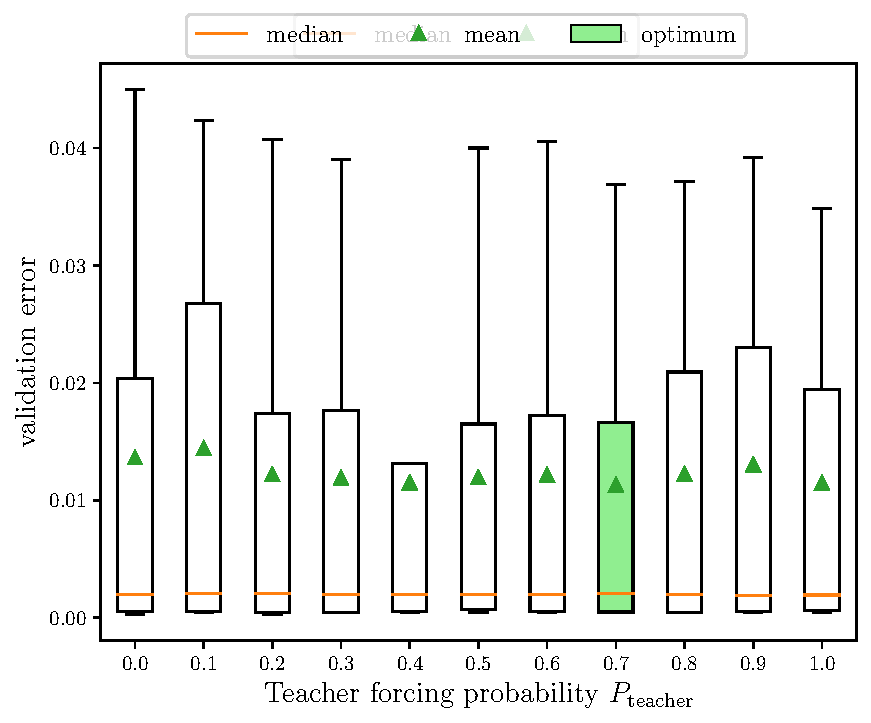
\includegraphics[width=0.5\textwidth]{box_plots/boxplot_teacher_forcing_opt.pdf}}%
				\only<4->{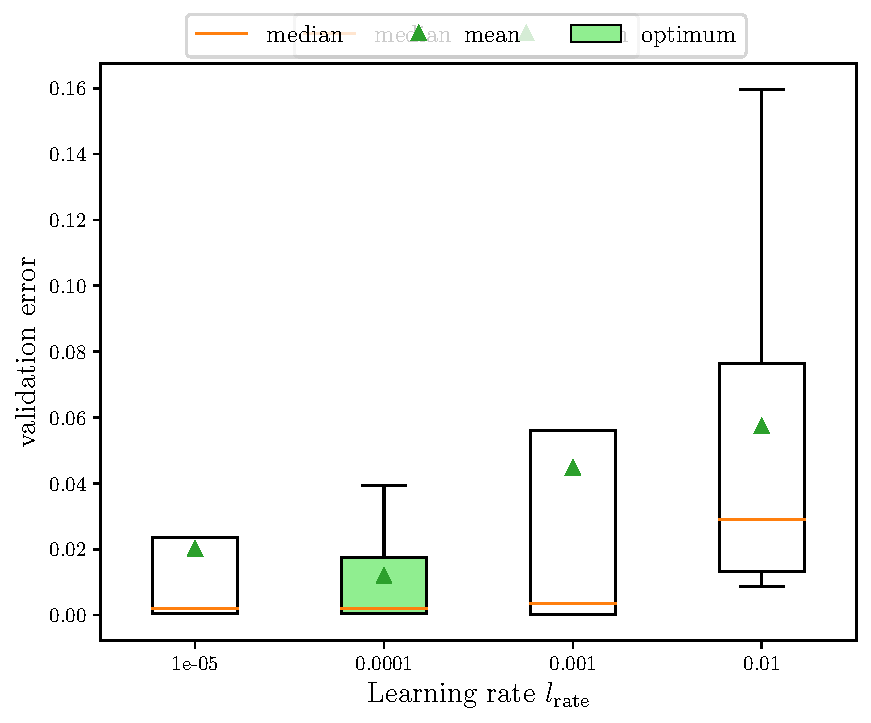
\includegraphics[width=0.5\textwidth]{box_plots/boxplot_learning_rate_opt.pdf}}%
			};
		\node [inner sep=0pt,above left, opacity=1.0]  at (1.01\textwidth,-0.7\textheight) (prediction) 
			{
				\only<1>{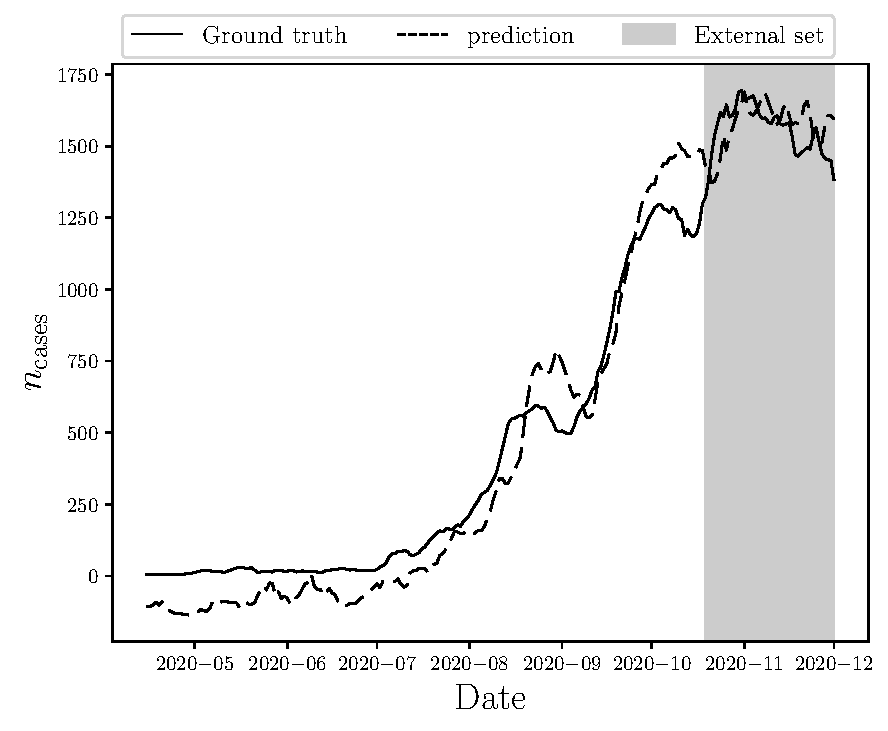
\includegraphics[width=0.5\textwidth]{models/final_model_n_layers.pdf}}%
				\only<2>{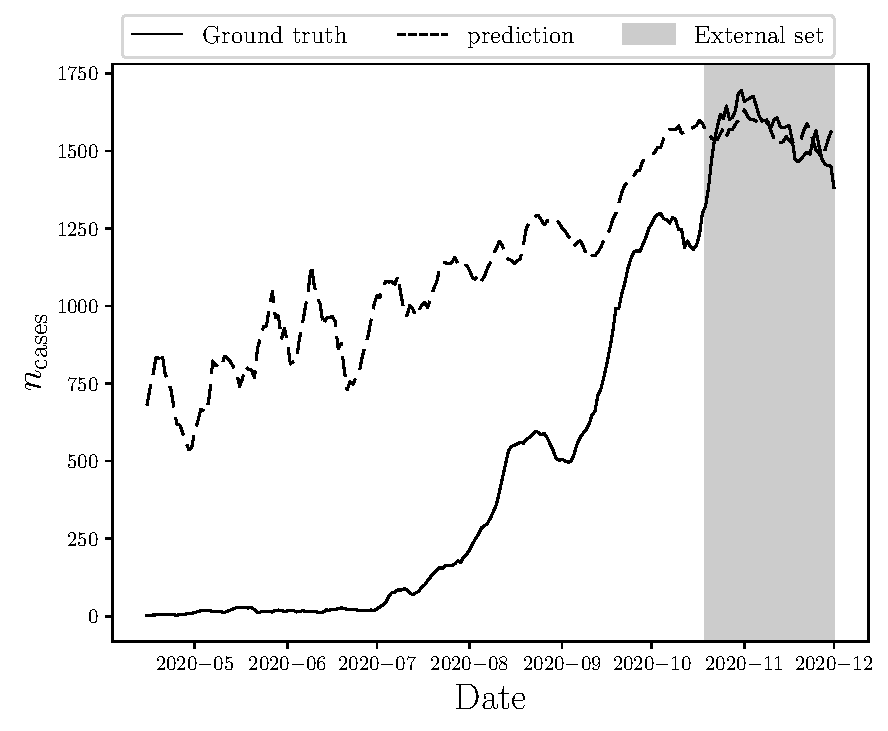
\includegraphics[width=0.5\textwidth]{models/final_model_batch_size.pdf}}%
				\only<3>{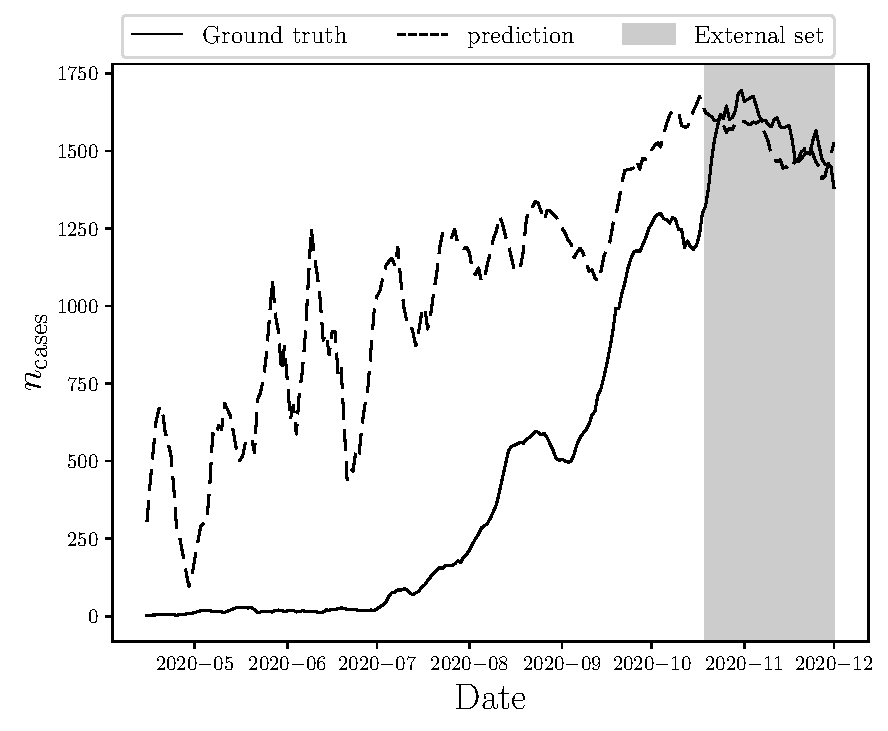
\includegraphics[width=0.5\textwidth]{models/final_model_teacher_forcing.pdf}}%
				\only<4->{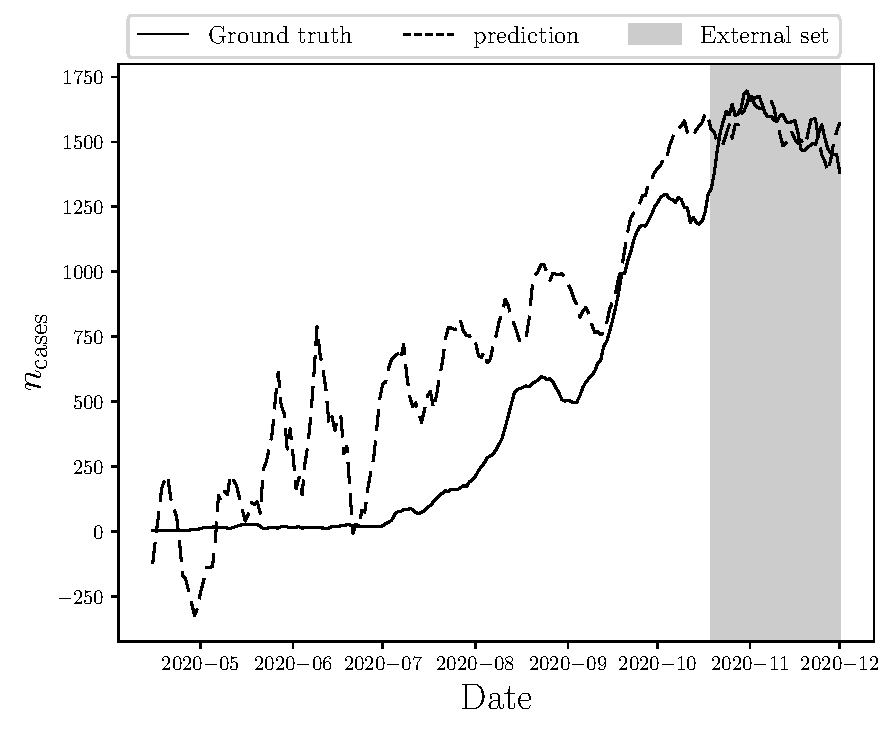
\includegraphics[width=0.5\textwidth]{models/final_model_learning_rate.pdf}}%
			};
		% show origin
		% \fill (0,0) circle (2pt);
	\end{tikzpicture}%
	%
	\vspace{-3em}
\end{frame}
\addtocounter{footnote}{-1}
%------------------------------------------------